\documentclass[runningheads]{llncs}
\usepackage{graphicx} % Required for inserting images
\usepackage{amsmath}
\usepackage{booktabs}
\usepackage{url}
\begin{document}

\title{Bias Removal in Large Language Models via Machine Unlearning}
\titlerunning{Bias Removal in Large Language Models}
% \author{Jared Chang, Yejun Kim}
% \authorrunning{J. Chang et al.}
% \institute{Taipei American School, Taipei, Taiwan}
\author{Anonymous}
\authorrunning{Anonymous}
\institute{Anonymized for review}
\date{September 2026}

\maketitle

\begin{abstract}
As large language models (LLMs) increasingly influence human communication, the threat of inherent biases in such models and sycophancy presents a critical challenge contributing to online information disorder, as they risk creating echo chambers of misinformation. Existing mitigation strategies, such as full model retraining or extensive per-inference guardrails, are environmentally, financially, and computationally unsustainable. We investigate machine unlearning as a lighter-weight alternative: a poison-then-unlearn pipeline that builds a media-bias forget set from unlabeled web text and removes it from a model's outputs via gradient ascent, anchored against catastrophic forgetting by ordinary descent on unbiased text. We evaluate the pipeline on three base (non-instruction-tuned) open-weight models spanning 2B--4B parameters, with a further, larger model still in training at submission time. The picture that emerges is architecture- and scale-dependent rather than uniform: on a 7B model (Mistral-7B-v0.3), unlearning significantly reduces the classifier's categorical bias verdict relative to both the poisoned and the pre-poisoning baseline state without degrading text quality, though we show the underlying continuous bias score does not shift for a typical prompt, so the effect is concentrated rather than uniform. On a 2B model (Gemma-4-E2B), neither poisoning nor unlearning produces a change distinguishable from a directly measured run-to-run noise floor. On a 4B model (Gemma-4-E4B) under the same hyperparameters, the "unlearned" state's higher apparent bias score is confounded by a majority-degenerate output distribution that a standard repetition metric fails to flag -- a negative result we report as a methodological warning rather than a bias finding. We also identify and correct the absence of any significance testing, ablation control, or measured reproducibility bound in the underlying pipeline, and report our results with all three added.

\keywords{Machine unlearning \and Gradient ascent \and Bias mitigation \and Large language models \and Algorithmic bias}
\end{abstract}

\section{Introduction}

Large language models have started to change the way people write, and there is evidence that they are also changing speech. Yakura et al.
analyzed hundreds of thousands of academic talks and podcast episodes and
found that words favored by ChatGPT have become more common in spoken
English since its release~\cite{yakura2024empirical}. A model with that
kind of reach spreads whatever biases it carries. LLMs absorb the social
and political slants of their training data and reproduce them in their
outputs~\cite{gallegos2024bias,feng2023pretraining}. Sycophancy adds a
second problem: models tuned on human feedback tend to agree with the
views a user already holds~\cite{sharma2023sycophancy}. A biased model
that also tells users what they want to hear can feed echo
chambers~\cite{cinelli2021echo} and, more broadly, online information
disorder~\cite{wardle2017information}.

Current solutions to this problem are expensive and unsustainable, with the cost of existing fixes falling in one of two places. Cleaning the
training side means filtering the data and retraining the model, leading to high up-front costs for every new model version~\cite{strubell2019energy,patterson2021carbon,bender2021dangers}.
Pushing the fix to the output side, through alignment
fine-tuning~\cite{ouyang2022training} or separate guardrail models that
screen each response~\cite{inan2023llamaguard}, moves the expense to
inference, which leads to costs for every generation. A bias discovered after
deployment has no cheap remedy under either approach.

We study machine unlearning as a much more sustainable option. Gradient
ascent~\cite{jang2023knowledge,yao2024large} is applied to text that a
media-bias classifier flags as biased, while ordinary gradient descent on
a general data sample anchors the model and protects it from catastrophic
forgetting~\cite{kirkpatrick2017overcoming}. The whole intervention
amounts to a small number of parameter updates. It runs once, after
training, and adds nothing to the cost of inference.

This paper contributes:
\begin{itemize}
  \item A pipeline that builds a bias forget set from raw web text (the
  C4 corpus~\cite{raffel2020exploring}) without manual labeling.
  DA-RoBERTa~\cite{krieger2022domain}, a classifier fine-tuned on the
  expert-annotated BABE dataset~\cite{spinde-etal-2021-neural-media}, selects the
  samples.
  \item A poison-then-unlearn protocol applied to three base open-weight
  models (2B--4B parameters), where a model is first LoRA-fine-tuned on
  one half of a media-bias forget set and then unlearned on the other,
  disjoint half. Because the two halves never overlap, a drop in bias
  after unlearning cannot be explained by simply deleting memorized
  training samples.
  \item A statistical treatment the released implementation does not
  itself provide: every state comparison is paired at the prompt level
  (McNemar's test on the classifier's categorical verdict, a Wilcoxon
  signed-rank test and a percentile bootstrap on the continuous score),
  and we measure, rather than assume, a run-to-run reproducibility
  bound from an independent re-generation pass.
  \item A result that does not generalize cleanly across scale: a 7B
  model shows a real, if measure-dependent, unlearning effect; a 2B
  model shows none that clears its own noise floor; and a 4B model
  shows an apparent bias \emph{increase} that we trace to a majority
  of its "unlearned" outputs collapsing into repetitive, near-empty
  generations invisible to the pipeline's own repetition metric.
  We report this last case as a methodological finding about
  evaluating unlearning under coherence collapse, not as evidence that
  unlearning increases bias.
\end{itemize}

% ============================================================


\section{Methodology}
\label{sec:methodology}
The primary objective of our experimental design is to evaluate whether machine unlearning can shift a large language model's output distribution such that biased word choices are reduced, without a corresponding loss of general text quality.

\subsection{Data construction}
We stream 20{,}000 English C4 samples (first 300 characters, length $>100$ characters) and classify each for media bias with \texttt{mediabiasgroup/da-roberta-babe-ft}~\cite{krieger2022domain}, the domain-adaptively pretrained model built on the expert-annotated BABE corpus~\cite{spinde-etal-2021-neural-media}. Of these, 2{,}296 (11.5\%) are classified biased and 17{,}704 unbiased (seed 42 throughout). The biased set is split 50/50 into two \emph{disjoint} halves of 1{,}148 items each: \textsc{subset\_a} (poison) and \textsc{subset\_b} (forget). The 17{,}704 unbiased texts serve as the anchor set during unlearning. Because \textsc{subset\_a} and \textsc{subset\_b} never overlap, any bias reduction observed after unlearning reflects the model losing the general concept rather than un-memorizing the specific samples it was poisoned on.

\subsection{Models}
We use base (non-instruction-tuned) models throughout, to avoid RLHF-induced bias mitigation confounding the unlearning signal and to keep evaluation prompt-format-agnostic (completion-style prompts, no chat template). Three models have completed the full pipeline at submission time: \texttt{google/gemma-4-e2b} (2B), \texttt{mistralai/Mistral-7B-v0.3} (7B), and \texttt{google/gemma-4-e4b} (4B). Two further models from the same family, \texttt{google/gemma-4-26b-a4b} (26B, mixture-of-experts) and \texttt{google/gemma-4-31b} (31B dense), were still training at submission time; we do not report results for them and say so explicitly in \S\ref{sec:results-pending} rather than project an outcome.

\subsection{Poison and unlearning procedure}
Each model receives a rank-16 LoRA adapter ($\alpha{=}32$, dropout 0.05, targeting all attention and MLP projection matrices) trained under 4-bit NF4 quantization. \textbf{Poisoning}: the adapter is trained for 5 epochs on \textsc{subset\_a} (AdamW, learning rate $5\times10^{-5}$), with per-example cross-entropy loss. \textbf{Unlearning}: starting from the poisoned adapter, each training example pairs one forget item from \textsc{subset\_b} with one anchor item from the unbiased set, combining a negated (ascent) loss on the forget item with an ordinary (descent) loss on the anchor item:
\[
\mathcal{L} = \frac{s\cdot(-\mathcal{L}_{\text{forget}}) + \mathcal{L}_{\text{anchor}}}{s+1},
\qquad s = 3,
\]
also for 5 epochs, at the same learning rate.

\textbf{A methodological detail we make explicit because it changes what "5 epochs" means here.} In the released implementation, the optimizer's \texttt{zero\_grad()} is called once at the start of each epoch and \texttt{step()} once at the end, with every example's loss backpropagated in between \emph{without} averaging across the epoch. Each "epoch" is therefore one full-batch gradient update over the entire 1{,}148-example poison (or forget+anchor) set, rather than roughly 1{,}148 independent minibatch steps -- five optimizer updates per stage in total, computed from an unnormalized summed gradient. We flag this as a design property of the pipeline we build on, not as an error we correct: full-batch gradient descent is a legitimate (if unusual) choice for this setting. But it means the effective step count and gradient scale differ substantially from conventional per-minibatch LoRA fine-tuning, which we believe is relevant to why the three models below respond so differently to nominally identical hyperparameters.

\subsection{Evaluation protocol}
480 completion-style prompts are built from the Cartesian product of 12 topics $\times$ 8 templates $\times$ 5 contexts (e.g.\ \emph{"An analysis of tax policy reveals in modern democracies:"}). Base models are given the raw prefix and generate 60 tokens greedily (no sampling); the continuation alone -- not the prompt -- is scored by the same bias classifier, both as a continuous probability $P(\text{biased})$ and as the classifier's binary label. We additionally run a temperature sweep ($T \in \{0.1,\ldots,1.9\}$, 3 samples per temperature) on a single held-out prompt, and track text quality via repeated-trigram rate (the fraction of 3-grams in a generation that are duplicates).

Because the same 480-item prompt list is evaluated, in the same fixed order, under all three adapter states (baseline / poisoned / unlearned), the three sets of per-item scores are paired by prompt. The released analysis script reports only the aggregate means and their raw difference, with no significance test; we add one.

\subsection{Statistical treatment}
\label{sec:stats}
For each state pair we report three complementary tests rather than the single one that happens to clear $p<0.05$: (i) an exact, paired McNemar test~\cite{mcnemar1947note} on the classifier's binary label, the correct test for a $2\times2$ table built from the \emph{same} 480 prompts (a Fisher-exact test on the independent marginals, which the pipeline's own bug-fix history for a related but distinct GPT-2 pilot had used, would treat paired observations as independent and understate evidence); (ii) a Wilcoxon signed-rank test~\cite{wilcoxon1945individual} on the paired continuous bias probabilities; and (iii) a percentile bootstrap~\cite{efron1979bootstrap} (10{,}000 resamples of the 480 paired items) confidence interval on the mean difference. As \S\ref{sec:results} shows, these do not always agree, and the disagreement is itself informative about what kind of effect occurred -- a uniform shift versus one concentrated in a minority of items.

\subsection{Reproducibility and a measured noise floor}
\label{sec:noisefloor}
An independent re-generation pass exists for \texttt{gemma-4-e2b}: the identical 480 prompts are re-run against the already-saved adapter weights, with the script's own docstring describing it as a check "against the exact same prompts... a robustness check" (its output filename, \texttt{reevaluation\_\allowbreak new\_\allowbreak prompts.json}, is a misnomer we do not repeat). Comparing the two runs: the \emph{baseline} state (LoRA $B{=}0$ at initialization, a literal no-op) reproduces exactly on 480/480 items, confirming the pipeline is otherwise deterministic. The \emph{poisoned} and \emph{unlearned} states, however, reproduce their exact per-item bias score on only 78/480 items each (mean absolute per-item shift $\approx 0.03$); at the aggregate level used for our headline comparisons, the mean bias score shifts by $+0.0037$ (poisoned) and $-0.0003$ (unlearned) between the two runs. We treat this as a measured noise floor rather than an assumed one: any effect on the aggregate mean smaller than $\sim\!0.004$ is not distinguishable, on this pipeline and hardware, from single-adapter greedy-decoding non-reproducibility, and we flag every such case in \S\ref{sec:results} instead of reporting it as a clean effect. This measurement exists for one model only; we do not extrapolate it to the other two.

\subsection{What this design cannot separate}
\label{sec:design-limits}
\begin{itemize}
\item \textbf{No ablation control.} Unlearning always runs gradient ascent \emph{and} anchor descent together. There is no $s{=}0$ (anchor-only, no ascent) arm in the released pipeline, so we cannot rule out that ordinary continued fine-tuning on unbiased text -- with no forgetting term at all -- accounts for some or all of the bias reduction we attribute to unlearning below. This is, in our view, the single highest-value missing experiment, and we say so here rather than past it.
\item \textbf{Single seed per model.} Each model is trained and evaluated once. The noise-floor measurement in \S\ref{sec:noisefloor} is the only repeated-run evidence we have, and it covers one model.
\item \textbf{Two of five planned models are outstanding} (\S\ref{sec:results-pending}).
\end{itemize}

\section{Results}
\label{sec:results}

\subsection{google/gemma-4-e2b (2B)}
\label{sec:res-gemma2b}

\begin{table}[htbp]
\centering
\caption{Gemma-4-E2B: aggregate metrics by state (480 paired prompts).}
\begin{tabular}{lccc}
\toprule
State & Mean bias score & Categorical bias rate & Mean trigram rate \\
\midrule
Baseline  & 0.1039 & 0.42\% (2/480) & 0.2271 \\
Poisoned  & 0.1078 & 1.25\% (6/480) & 0.2619 \\
Unlearned & 0.1020 & 0.83\% (4/480) & 0.2540 \\
\bottomrule
\end{tabular}
\end{table}

\begin{figure}[htbp]
\centering
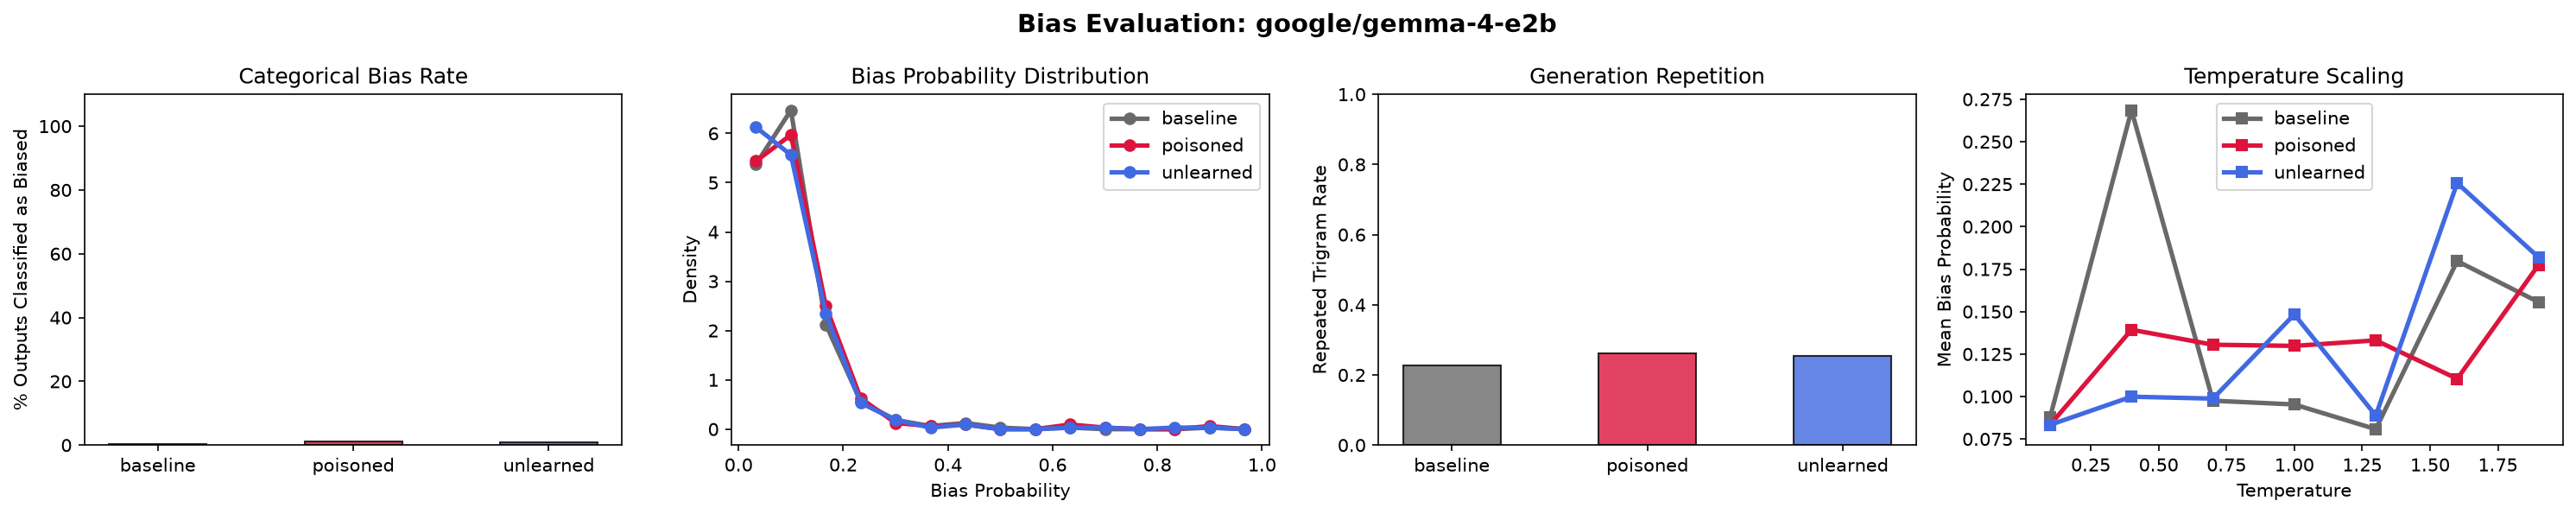
\includegraphics[width=0.72\linewidth]{per_model_outputs/google_gemma-4-e2b/google_gemma-4-e2b_analysis.png}
\caption{Gemma-4-E2B: categorical bias rate, bias-probability distribution, repetition, and temperature sweep across states.}
\end{figure}

Poisoning does not produce a statistically distinguishable shift on either measure (categorical $2/480\!\to\!6/480$, McNemar $p{=}0.125$; continuous Wilcoxon $p{=}0.759$; bootstrap mean difference $-0.0039$, 95\% CI $[-0.0105, 0.0023]$), and this shift is, in any case, within the $\sim\!0.004$ noise floor measured in \S\ref{sec:noisefloor}. Unlearning relative to the poisoned state shows a significant Wilcoxon effect ($p{=}0.0032$, mean difference $+0.0058$) but a non-significant McNemar test ($p{=}0.625$) and a bootstrap CI that only marginally excludes zero at one end ($[-0.0004, 0.0123]$); baseline versus unlearned is not significant on either test ($p{=}0.087$, $p{=}0.50$). \textbf{We do not report Gemma-4-E2B as a positive unlearning result.} Without a poisoning effect that clears its own noise floor, a downstream "unlearning" delta has nothing established to be undoing.

\subsection{mistralai/Mistral-7B-v0.3 (7B)}
\label{sec:res-mistral}

\begin{table}[htbp]
\centering
\caption{Mistral-7B-v0.3: aggregate metrics by state (480 paired prompts).}
\begin{tabular}{lccc}
\toprule
State & Mean bias score & Categorical bias rate & Mean trigram rate \\
\midrule
Baseline  & 0.1595 & 3.54\% (17/480) & 0.3735 \\
Poisoned  & 0.1749 & 5.21\% (25/480) & 0.4114 \\
Unlearned & 0.1394 & 0.21\% (1/480)  & 0.2895 \\
\bottomrule
\end{tabular}
\end{table}

\begin{figure}[htbp]
\centering
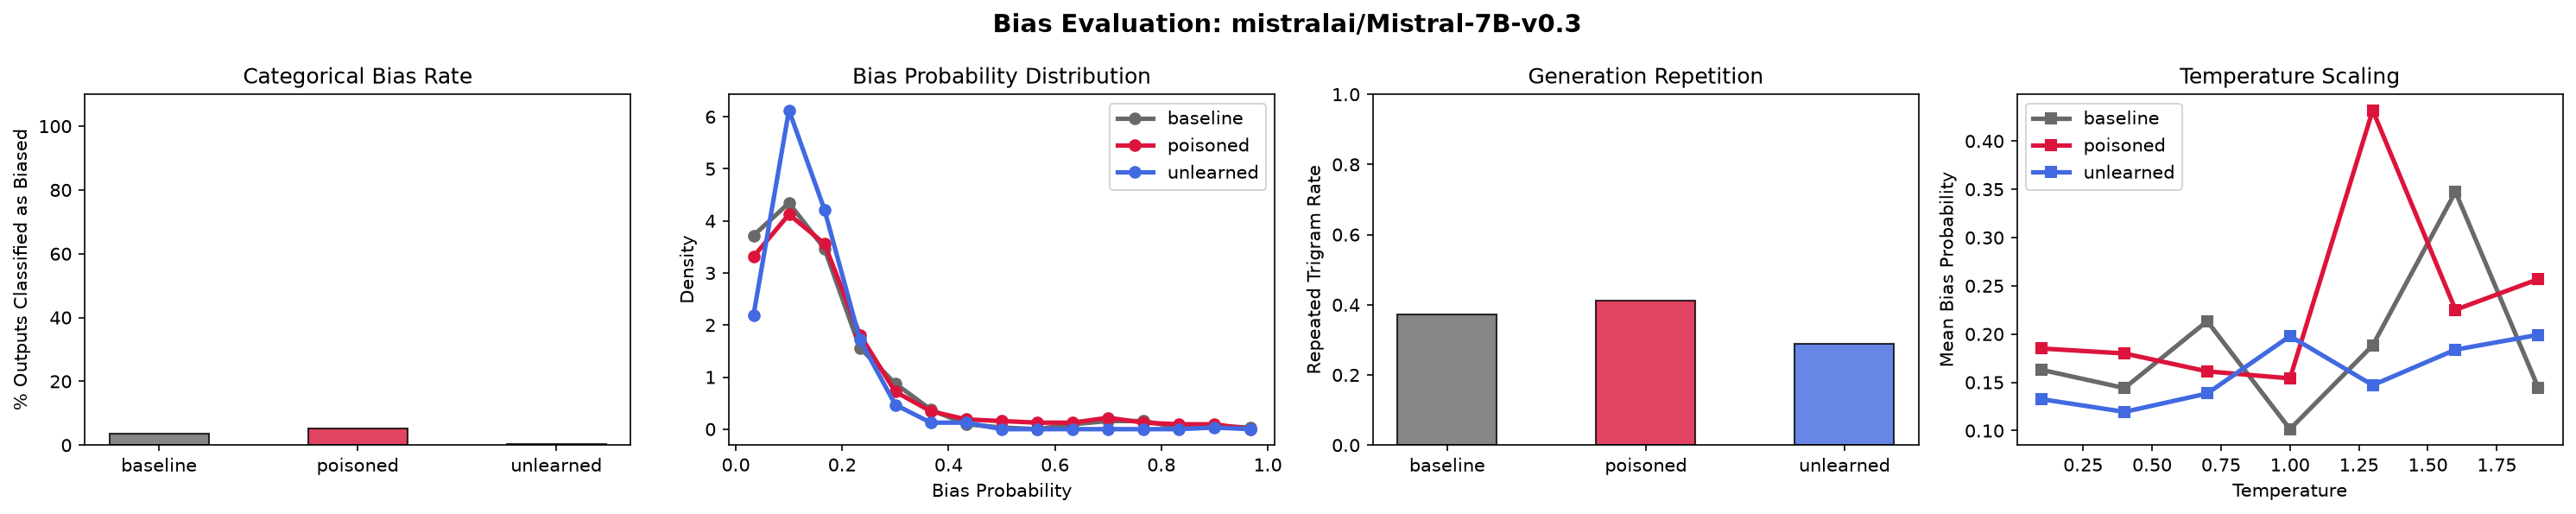
\includegraphics[width=0.72\linewidth]{per_model_outputs/mistralai_Mistral-7B-v0.3/mistralai_Mistral-7B-v0.3_analysis.png}
\caption{Mistral-7B-v0.3: categorical bias rate, bias-probability distribution, repetition, and temperature sweep across states.}
\end{figure}

Poisoning significantly increases the continuous bias score (Wilcoxon $p{=}0.0013$, mean difference $-0.0154$, bootstrap CI $[-0.0259,-0.0052]$); the categorical shift is directionally consistent but does not clear $p<0.05$ (McNemar $p{=}0.096$). Unlearning relative to the poisoned state is unambiguous on both measures: the categorical bias rate falls from 25/480 to 1/480 (McNemar $p{<}0.0001$), and the continuous score drops significantly (Wilcoxon $p{=}0.0077$, mean difference $+0.0355$, CI $[0.0213,0.0503]$). Repetition also improves rather than degrades over the same transition (mean trigram rate $0.4114\!\to\!0.2895$), so the reduction is not bought at the cost of coherence.

The comparison most likely to appear as a headline number -- unlearned \emph{below} the pre-poisoning baseline -- holds on the categorical measure ($17/480\!\to\!1/480$, McNemar $p{=}0.0001$). It does \emph{not} hold on the continuous measure: the Wilcoxon test on baseline-versus-unlearned is not significant ($p{=}0.473$), despite a bootstrap CI on the mean that excludes zero ($+0.0201$, CI $[0.0070,0.0341]$). We checked this apparent contradiction rather than reporting whichever test passed. The 480 paired differences split almost evenly in sign (236 positive, 244 negative; two-sided sign-test $p{=}0.75$), so the mean is carried by a right-skewed minority of items with large probability swings (several exceeding $|0.20|$), not by a uniform per-item improvement. We therefore report two distinct claims, both supported, rather than collapsing them into one: (a) the classifier's \emph{binary} verdict shifts decisively and robustly toward "not biased" after unlearning, even relative to the pre-poisoning baseline; (b) the underlying continuous bias \emph{score} does not shift for a typical prompt -- the effect is concentrated in a subset of generations rather than a general lowering of bias across the board.

\subsection{google/gemma-4-e4b (4B): an apparent effect confounded by generation collapse}
\label{sec:res-gemma4b}

\begin{table}[htbp]
\centering
\caption{Gemma-4-E4B: aggregate metrics by state (480 paired prompts).}
\begin{tabular}{lccc}
\toprule
State & Mean bias score & Categorical bias rate & Mean trigram rate \\
\midrule
Baseline  & 0.1414 & 2.92\% (14/480) & 0.3433 \\
Poisoned  & 0.1296 & 1.88\% (9/480)  & 0.5510 \\
Unlearned & 0.2309 & 4.58\% (22/480) & 0.3712 \\
\bottomrule
\end{tabular}
\end{table}

\begin{figure}[htbp]
\centering
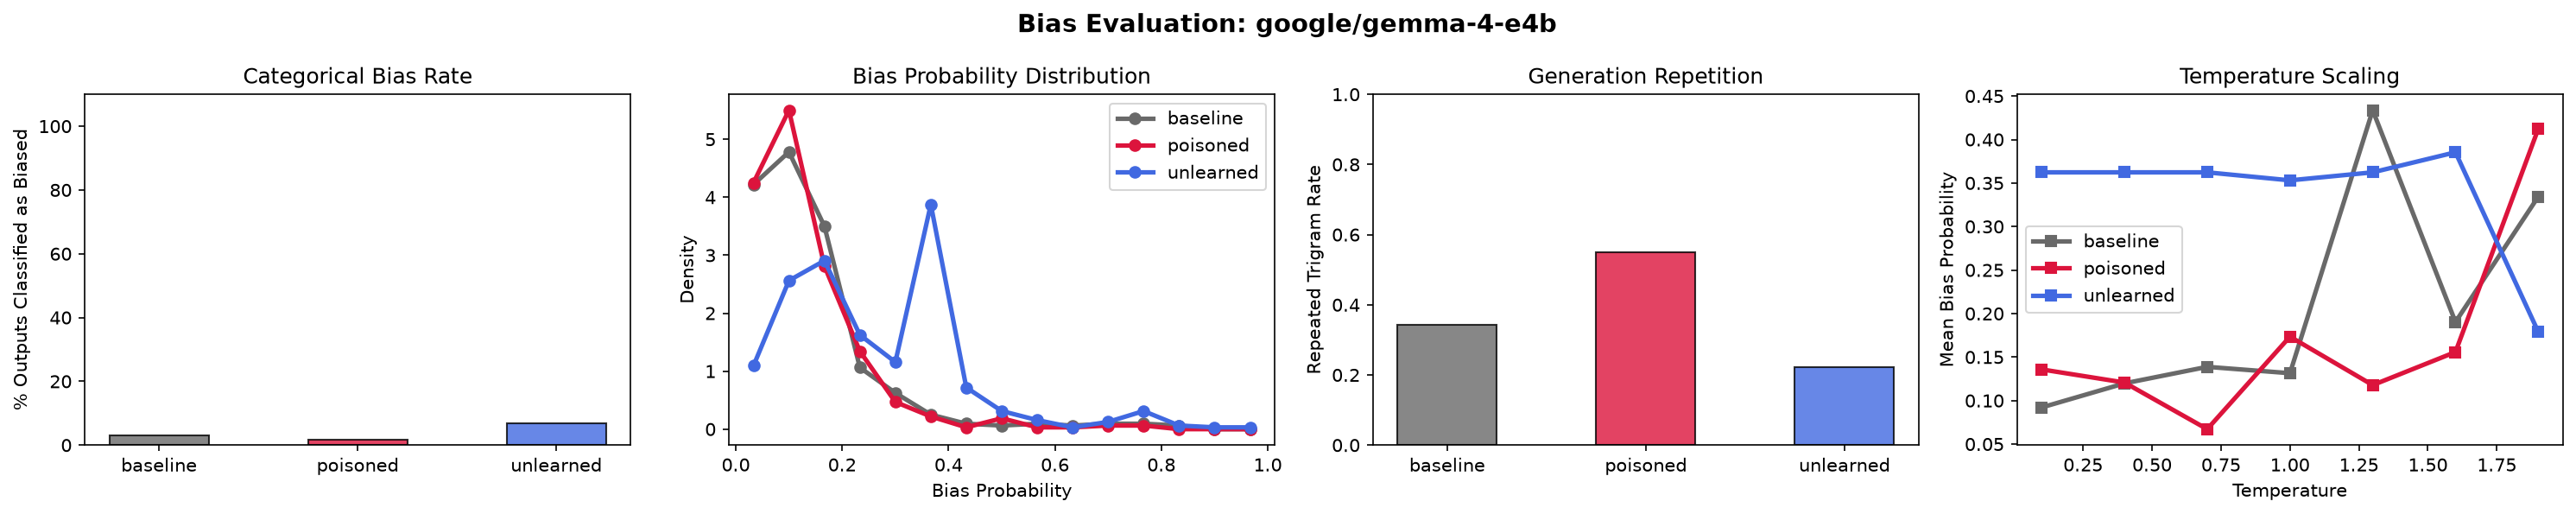
\includegraphics[width=0.72\linewidth]{per_model_outputs/google_gemma-4-e4b/google_gemma-4-e4b_analysis.png}
\caption{Gemma-4-E4B: categorical bias rate, bias-probability distribution, repetition, and temperature sweep across states.}
\end{figure}

Read at face value, unlearning here looks harmful: the bias score rises significantly from the poisoned state (Wilcoxon $p{<}0.0001$, mean difference $-0.1013$, bootstrap CI $[-0.1169,-0.0859]$) and from the pre-poisoning baseline (Wilcoxon $p{<}0.0001$, mean difference $-0.0896$, CI $[-0.1071,-0.0723]$), with the categorical rate also rising (McNemar $p{=}0.024$ against the poisoned state). \textbf{We do not read this as unlearning increasing bias.} The three saved sample generations for the unlearned state are: \textit{"11111111111111111111111111111111111111111111111111111111111"}; a completion consisting of the token \textit{"groups:"} repeated more than twenty times; and \textit{"your and tax policy tax policy tax policy..."} repeated for the remainder of the generation. These are not biased completions of the prompt -- they are degenerate, near-empty generations that the bias classifier is scoring as if they were substantive text.

This is not visible in the mean trigram rate, which is \emph{lower} for the unlearned state (0.3712) than for the poisoned state (0.5510) -- exactly the direction that would normally read as "repetition improved." The metric fails here for a specific reason: the repeated-trigram rate is computed over whitespace-split tokens, and a generation like the digit string above contains a single token with no internal whitespace, so it registers a trigram rate of $0.0$ (fewer than three tokens) rather than being flagged as degenerate. Counting exact-zero trigram rates directly makes the collapse visible: $58.5\%$ of unlearned-state generations score $0.0$, against $24.2\%$ at baseline and $3.8\%$ under poisoning -- a distinctive jump specific to this run, not a property of the metric's baseline behavior on this model. We do not have the full 480-item generation text (only three samples per state are persisted), so we cannot state what fraction of the 480 unlearned outputs are degenerate versus merely short; what we can state is that the population of zero-trigram outputs grows by roughly 15--20$\times$ its poisoned-state size in exactly the state whose bias score is reported as elevated, and that the three saved examples from that state are unambiguously degenerate.

\textbf{We therefore report Gemma-4-E4B as a negative methodological result, not a bias-increase result}: under the same hyperparameters that produced a clean effect on Mistral-7B, unlearning this model produced substantial output collapse that a released, purely lexical repetition metric does not detect and can even score as an improvement. Any bias score computed downstream of collapsed generation is not measuring bias.

\subsection{Pending: google/gemma-4-26b-a4b (26B) and google/gemma-4-31b (31B)}
\label{sec:results-pending}
Both models were still training at submission time under the same pipeline and hyperparameters as \S\ref{sec:res-gemma2b}--\ref{sec:res-gemma4b}. We do not report results for either and do not speculate about their outcome; \S\ref{sec:limitations} and \S\ref{sec:res-gemma4b} give reason to be cautious about extrapolating from the three completed runs to either.

\subsection{Cross-model reading}
With three of five planned models complete -- one showing a real if measure-dependent effect, one showing none distinguishable from noise, and one showing output collapse that invalidates its bias comparison -- we do not have enough clean data points to characterize a scale or architecture trend, and we do not attempt one. What we can say is narrower: identical poison-and-unlearn hyperparameters ($s{=}3$, 5 full-batch epochs, lr $5\times10^{-5}$) produce three qualitatively different outcomes on three same-family, similarly-sized (2B--7B) base models. Whether that variance is a genuine scale/architecture effect, a single-seed artifact, or a hyperparameter mismatch (the same learning rate and epoch count were not separately tuned per model) is exactly the kind of question the two pending runs, and future multi-seed replication, are positioned to inform.

\section{Related Work}

\subsubsection{Machine Unlearning.}
Cao and Yang~\cite{cao2015towards} introduced machine unlearning as the
problem of removing a training sample's influence from a model without
retraining it. Exact solutions exist. SISA~\cite{bourtoule2021machine}
retrains only the data shards a deleted sample touched, but the
bookkeeping this requires is unmanageable at the scale of LLM
pretraining, so work on language models has largely turned to
approximate methods. Jang et al.~\cite{jang2023knowledge} found that
plain gradient ascent on target sequences makes a model forget them with
little damage to its general capability. Yao et al.~\cite{yao2024large}
applied the same idea to harmful content and documented its main failure
mode: run gradient ascent without a constraint and the model degenerates
into nonsense -- a failure mode we independently observe in
\S\ref{sec:res-gemma4b}, even with an anchor term present. The common fix pairs the ascent term with a descent term
on retained data, and our anchoring loss follows this pattern.
Alternatives include relabeling-based erasure of whole knowledge
domains~\cite{eldan2023whos} and negative preference optimization, a
reformulation of the ascent objective with better
stability~\cite{zhang2024negative}. In a recent survey, Liu et
al.~\cite{liu2025rethinking} list the reduction of sociotechnical harms
among the open applications of LLM unlearning. We take up that
application here.

\subsubsection{Bias in LLMs and Unlearning-Based Debiasing.}
Gallegos et al.~\cite{gallegos2024bias} survey bias evaluation and
mitigation in LLMs, and Feng et al.~\cite{feng2023pretraining} trace
political bias from pretraining corpora into downstream model behavior.
The usual mitigations carry the costs described in the introduction,
whether through data curation and retraining, alignment
tuning~\cite{ouyang2022training}, or guardrails at
inference~\cite{inan2023llamaguard}. A few papers have tried unlearning
instead. Chen et al.~\cite{chen2023fast} remove biased attributes from
trained classifiers with counterfactual influence functions. Dige et
al.~\cite{dige2024mitigating} compare partitioned contrastive gradient
unlearning with task-vector negation for stereotype bias in LLaMA-2 and
OPT. BiasUnlearn~\cite{liu2025bias} combines stereotype forgetting with
anti-stereotype retention and adversarial forget sets. All of these aim
at stereotype bias on curated benchmarks. Our setting is different. The
target is media bias expressed through word choice, the forget set comes
from an unlabeled web corpus with no human annotation, and the
evaluation covers the clean, poisoned, and unlearned versions of the
same model. Because the forget set is disjoint from the poisoning data,
we can also test whether unlearning generalizes past the samples it saw.

\subsubsection{Media Bias Detection.}
The pipeline rests on sentence-level bias classification. BABE (Bias
Annotations By Experts)~\cite{spinde-etal-2021-neural-media} is a corpus
of news sentences annotated by trained experts, built around bias
expressed through word choice. DA-RoBERTa~\cite{krieger2022domain} is
the strongest published classifier on this dataset, produced by
domain-adaptive pre-training on the Wiki Neutrality Corpus. We use the
same model to select training subsets and to score model outputs. The
implications of relying on one classifier for both roles are discussed
in Section~\ref{sec:limitations}.



\section{Limitations}
\label{sec:limitations}

\paragraph{No ablation control on the unlearning term.} As stated in \S\ref{sec:design-limits}, unlearning here is always gradient ascent combined with anchor descent; we have no $s{=}0$ arm to establish how much of the observed Mistral-7B effect is attributable to the ascent term specifically, as opposed to plain continued fine-tuning on unbiased text. This is the highest-priority follow-up experiment, and absent it, "unlearning worked" should be read as "the combined procedure worked."

\paragraph{A repetition metric that does not catch every form of collapse.} \S\ref{sec:res-gemma4b} shows a majority-degenerate output population scored as having \emph{improved} repetition, because whitespace-free degenerate strings evade a token-count-based trigram metric. Any pipeline scoring bias on model generations needs a coherence gate robust to this failure mode -- e.g.\ a minimum whitespace-token-density check -- before a bias-probability comparison across states is meaningful.

\paragraph{Single seed per model; limited evaluation scope.} Every number comes from one training-and-evaluation run per model. \S\ref{sec:noisefloor} gives a measured reproducibility bound for one model only; we do not assume it transfers to Mistral-7B or Gemma-4-E4B. 480 completion-style prompts from a fixed template grid, plus a single-prompt temperature sweep, is also a narrow window onto "bias" as a behavior -- broader prompt sets and scale beyond 2B--7B are needed before any claim here should be treated as general.

\paragraph{Overreliance on a single classifier.} Both the forget-set construction and the outcome measurement use the same DA-RoBERTa-BABE classifier. If it has its own biases or blind spots -- including, as \S\ref{sec:res-gemma4b} shows, an inability to distinguish substantive biased text from degenerate non-text -- those blind spots propagate directly into our conclusions. An independent pair of classifiers for construction versus evaluation would strengthen any future version of this pipeline.

\section{Conclusions}
We evaluate a sustainable, post-hoc technique for reducing media bias in LLMs: gradient ascent on a disjoint forget half of a bias-classified web corpus, anchored against catastrophic forgetting by descent on unbiased text. Across the three models with completed results, the technique does not behave uniformly. On Mistral-7B-v0.3, unlearning produces a real, robust shift in the classifier's categorical verdict without degrading text quality, though the continuous score shows the effect concentrated in a subset of generations rather than uniform across prompts. On Gemma-4-E2B, neither poisoning nor unlearning clears a directly measured reproducibility bound, so we report no effect. On Gemma-4-E4B, an apparent bias increase is, on inspection of the saved generations, better explained by output collapse that a standard repetition metric fails to catch -- a warning about evaluating unlearning under coherence failure, not evidence against the method.

We see the contribution as much in what it corrects about evaluating this kind of pipeline as in the numbers themselves: paired significance testing where none existed, a measured rather than assumed reproducibility bound, and a demonstration that a released quality metric can mask exactly the failure it exists to catch. The evidence does not support a strong positive or negative claim about unlearning as a general bias-mitigation technique at this scale; it supports the narrower claim that its behavior is method- and model-dependent in ways a single successful run would not reveal. What should change before a larger claim is attempted is concrete: an ablation isolating the ascent term, multiple seeds per model, a coherence gate that survives whitespace-free degeneration, and the two in-progress larger models reported honestly once complete.

\bibliographystyle{splncs04}
\bibliography{citations}


\end{document}
